\chapter{Realisierung des Source-To-Source Compilers}
\label{chap:Realisierung}

Basierend auf der Einführung zu Compilern und den Herausgearbeiteten Unterschieden zwischen Xamarin.Forms und Flutter sowie der verwendeten Programmiersprachen \Csharp und Dart kann in diesem Kapitel die Realisierung des Source-To-Source Compilers beschrieben werden. 

\section{Entwicklungsumgebung}
Für die Realisierung sind verschiedene Softwarekomponenten erforderlich,  die zum einen für die Entwicklung und zum anderen für die Qualitätssicherung eingesetzt werden.  Wie bereits in Kapitel \ref{chap:CompilerEntwurf} beschrieben,  soll für einen Teil der zu Übersetzung der Rosyln Compiler von Microsoft verwendet werden.  Um Projekte mit Roslyn Integration zu implementieren bietet sich die Entwicklungsumgebung (engl.  \ac{ide}) Visual Studio 2019 an.  Da auf dieser  Plattform Projekte angelegt werden können,  die mit dem Roslyn Compiler Interagieren.  Zusätzlich können in Visual Studio auch grafische Benutzeroberflächen und Xamarin.Forms Anwendungen realisiert werden.  Die zu programmierende Projektmappe kann demnach aus den folgenden frei Projekten bestehen.  Des Source-To-Source Compilers mit Roslyn Integration, der grafischen Benutzeroberfläche und einer Xamarin.Forms Anwendung anhand welcher der Prototyp validiert werden kann.  Neben der \ac{ide} bilden die sogenannten Build tools for Visual Studio einen wichtigen Bestandteil des Compilers da diese es erlauben \Csharp -Projekte zu kompilieren.  Damit der Compiler Flutter Projekte angelegen kann wird die Flutter \ac{sdk} als Abhängigkeit des Compilers benötigt.  Um die übersetzte Flutter App anschließend testen zu können bietet es sich ebenfalls an eine Flutter- \ac{ide} zu installieren dafür kann auf Visual Studio Code oder Android Studio zurückgegriffen werden.  In Abbildung \ref{fig:IDE} wird die Systemlandschaft des zu entwickelnden Compilers visualisiert. 



\begin{figure}[!ht]
 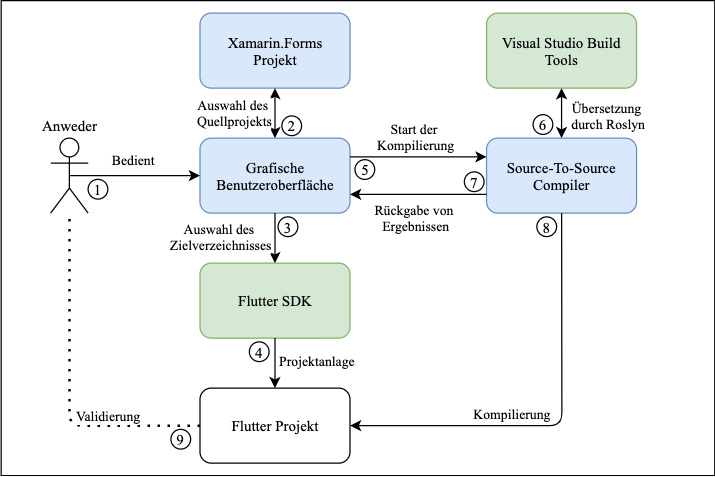
\includegraphics[width=\textwidth,keepaspectratio]{Images/Implementation/IDE.png}
 \caption{Source-To-Source Compiler Informationsfluss}
 \label{fig:IDE}
\end{figure}
In der Abbildung werden die in dieser Arbeit zu realisierenden Komponenten in Blau dargestellt,  die Visual Studio Build Tools und die Flutter \ac{sdk} werden jeweils in grün dargestellt da es sich dabei um bereits existierende Softwarekomponenten handelt.  Da die Build Tools ausschließlich für Windows Computer zur Verfügung stehen wird der zu entwickelnde Übersetzer ebenfalls nur auf Windows Computern lauffähig sein.  auf der Abbildung sind die jeweiligen Interaktionen mit zahlen versehen,  welche die Reihenfolge in der Abarbeitung skizzieren soll.  So wählt der Anwender das Xamarin.Forms Projekt aus und anschließend das Zielverzeichnis indem mit Hilfe der Flutter SDK das Projekt imitiert wird.  Anschließend werden diese Informationen an den Source-To-Source Compiler übergeben, welcher zusammen mit den Visual Studio Build Tools das Ausgangsprojekt übersetzt und die Ergebnisse zurück an die \ac{gui} leitet.  Außerdem werden die übersetzten Dart dateien im angelegten Dart Projekt abgelegt werden und der Anwender kann das Flutter Projekt testen.  
In den folgenden Unterabschnitten werden sowohl die Entwicklung der grafische Benutzeroberfläche, als auch des Source-To-Source Compilers beschrieben.  Das Xamarin.Forms Projekt, welche für diese Arbeit angelegt wird, wird in Kapitel \ref{chap:Qualitätssicherung} behandelt. 



\section{Metadaten}


Mit Hilfe von Roslyn konnte der Name des Projektes extrahiert werden.  Dieser Name kann anschließend verwendet werden um ein neues Flutter Projekt zu initialisieren.  

Wie der Quelltext zeigt,  wird dafür ein neues Projekt mit Hilfe der Kommandozeile angelegt.  Damit das Ergebnis nicht von vorherigen Übersetzungsvorgängen beeinträchtigt wird,  auch im Vorhinein überprüft,  ob das Zielverzeichnis existiert und leer ist. 

\section{XAML zu Dart}

\section{C\# zu Dart}


Da sowohl die grafische Benutzeroberfläche als auch der Source-To-Source Compiler mit .Net Technologien realisiert wurden lassen sie sich einfach miteinander kombinieren.  Dafür erhält die  \ac{gui} eine Ahängigkeit auf das \ac{s2s}-Projekt.  



\section{Grafische Benutzeroberfläche}
Die \ac{gui} ist der zentrale Berührungspunkt von Anwendern mit dem Source-To-Source Compiler.  Er spielt soll die notwendigen Eingabe-Möglichkeiten anbieten,  das Ergebnis ausgeben und den Anwender auf mögliche Fehler hinweisen.  Als grafisches Vorbild soll auf das in Kapitel \ref{chap:CompilerEntwurf} entworfene Mockup zurückgegriffen werden.  Für die Erstellung einer grafischen Benutzeroberfläche stehen eine Vielzahl von Technologien mit verschiedenen Vor- und Nachteilen zur Verfügung.  Beispielsweise hätte eine Webseite den Vorteil,  das Anwender keinen Installationsaufwand haben und darüber hinaus auch Plattform-unabhängig auf den Compiler zugreifen können.  Jedoch bringen Webseiten neben dem eigentlichen Entwicklungsaufwand weitere Herausforderungen mit sich,  so haben potentielle Anwender nicht mehr die volle Kontrolle über ihren eigenen Quelltext, wenn sie diesen auf einer Webseite hochladen.  
Aus diesem Grunde,  wird die in dieser Arbeit entworfene Oberfläche eine lokale Anwendung sein,  die von Anwendern lokal installiert werden muss aber im Gegenzug garantiert,  dass niemand Zugriff auf den Source-Code von Anwendern erhält.  Zu diesem Zwecke wird die \ac{gui} mit der Technologie \ac{wpf} realisiert.  Dabei handelt es sich um ein \ac{ui}-Framework des .NET Frameworks welches für die Erstellung von Desktop Anwendungen geeignet ist und mit XAML und \Csharp entwickelt wird.  \footcite[Vgl.][S. 1f]{Wenger2012} Da die Build Tools für Visual Studio nur für Windows Computer ist es auch keine Einschränkung,  dass Anwendungen die mit \ac{wpf} realisiert werden ausschließlich unter diesem Betriebssystem ausführbar sind.

In der Zukunft könnte der Source to Source Compiler auch eine Web-Oberfläche bekommen,  diese hätte die zwei folgenden essentielle Vorteile im Gegensatz zu der aktuellen Implementierung.  Reduktion des Installationsaufwandes - durch den Betrieb über eine Webseite könnte die Installation von der Anzeige entkoppelt werden.  Natürlich wäre eine Client-Server Struktur auch ohne eine Webseite erreichbar,  jedoch haben Webseiten darüber hinaus den zusätzlichen Vorteil,  dass sie Plattform-unabhängig zur Verfügung stehen,  was es zum Beispiel für Xamarin.Forms Entwickelr mit einem Mac OSX Computer erlauben würde ebenfalls von dem Compiler zu profitieren, ohne sich eine Windows Installation vornehmen zu müssen
